\chapter{Technical Foundation}\label{chap:technical-foundation}  % other option are Framework Design, Implementation Details

In this chapter, we provide a comprehensive description of the context composition framework, which is applied to preprocess the data as reported in the subsequent section. We then present the fine-tuning pipeline, a tool that integrates this data to facilitate the project adaptation of Code LLMs. Additionally, a list of tools necessary for executing these implementations is included.

The contributions outlined in this chapter are: the context composition framework with 13 different composers implemented, a set of pre-composed training datasets, and a fine-tuning pipeline.

\section{Context Composition Framework}

We begin this section with an explanation of the independent building blocks of the context composition framework and their integration to form a complete compositional strategy. The chapter then enumerates all the composers utilized in the experimental section, accompanied by their descriptions. Finally, we offer an overview of the additional parameter applied to modify the retrieval order and include a commentary that invites further exploratory investigation into the framework.

\subsection{Building Blocks}

As stated in \sectionref{sec:training-stages}, we define the context composer as a function that takes a repository snapshot and a completion file and returns a string that represents the project context. The investigation of ICL capabilities requires a diverse array of such functions. Therefore, we conclude that the most effective strategy to achieve this diversity is to decompose the context composers into atomic pieces that can be repeatedly utilized. We propose seven abstract building blocks for this framework:

\begin{enumerate}
    \item \textbf{File Filtering} determines which files to include in the subsequent data processing pipeline. For instance, it can filter out files with empty content or files with certain extensions.
    \item \textbf{File Preprocessing} modifies the content of the files. For example, it can extract code from markdown files.
    \item \textbf{File Chunking} changes the granularity of the data from files to text chunks. The simplest form of chunking is identity, which maintains the file-grained structure.
    \item \textbf{Chunk Ranking} determines the relevance of the chunks for the completion file. It can take multiple forms, ranging from simple heuristics and sparse embedding comparisons to more sophisticated dense approaches.
    \item \textbf{Chunk Sorting} defines the rules for ordering the chunks based on their ranks. The most common scenario is to sort the chunks in ascending order of their ranks, placing the most relevant chunks at the end of the list.
    \item \textbf{Chunk Assembling} joins sorted chunks into a single string using a specific template. For example, the assembler can prepend a comment with path information of the chunk's source file and join them using a separator string.
    \item \textbf{Context Postprocessing} modifies the context as a unified string. For instance, line dropout can be applied by this block.
\end{enumerate}

Each of these blocks has its own abstract class and serves as a foundation for concrete implementations. This design allows for several different transformations associated with a single block type to be part of a single context composer, eliminates code duplication and allows for greater flexibility in composer creation. We present the directed graph in \figureref{fig:composer-blocks} that visualizes the order in which these instances can be applied.

\begin{figure}[ht]
    \centering
    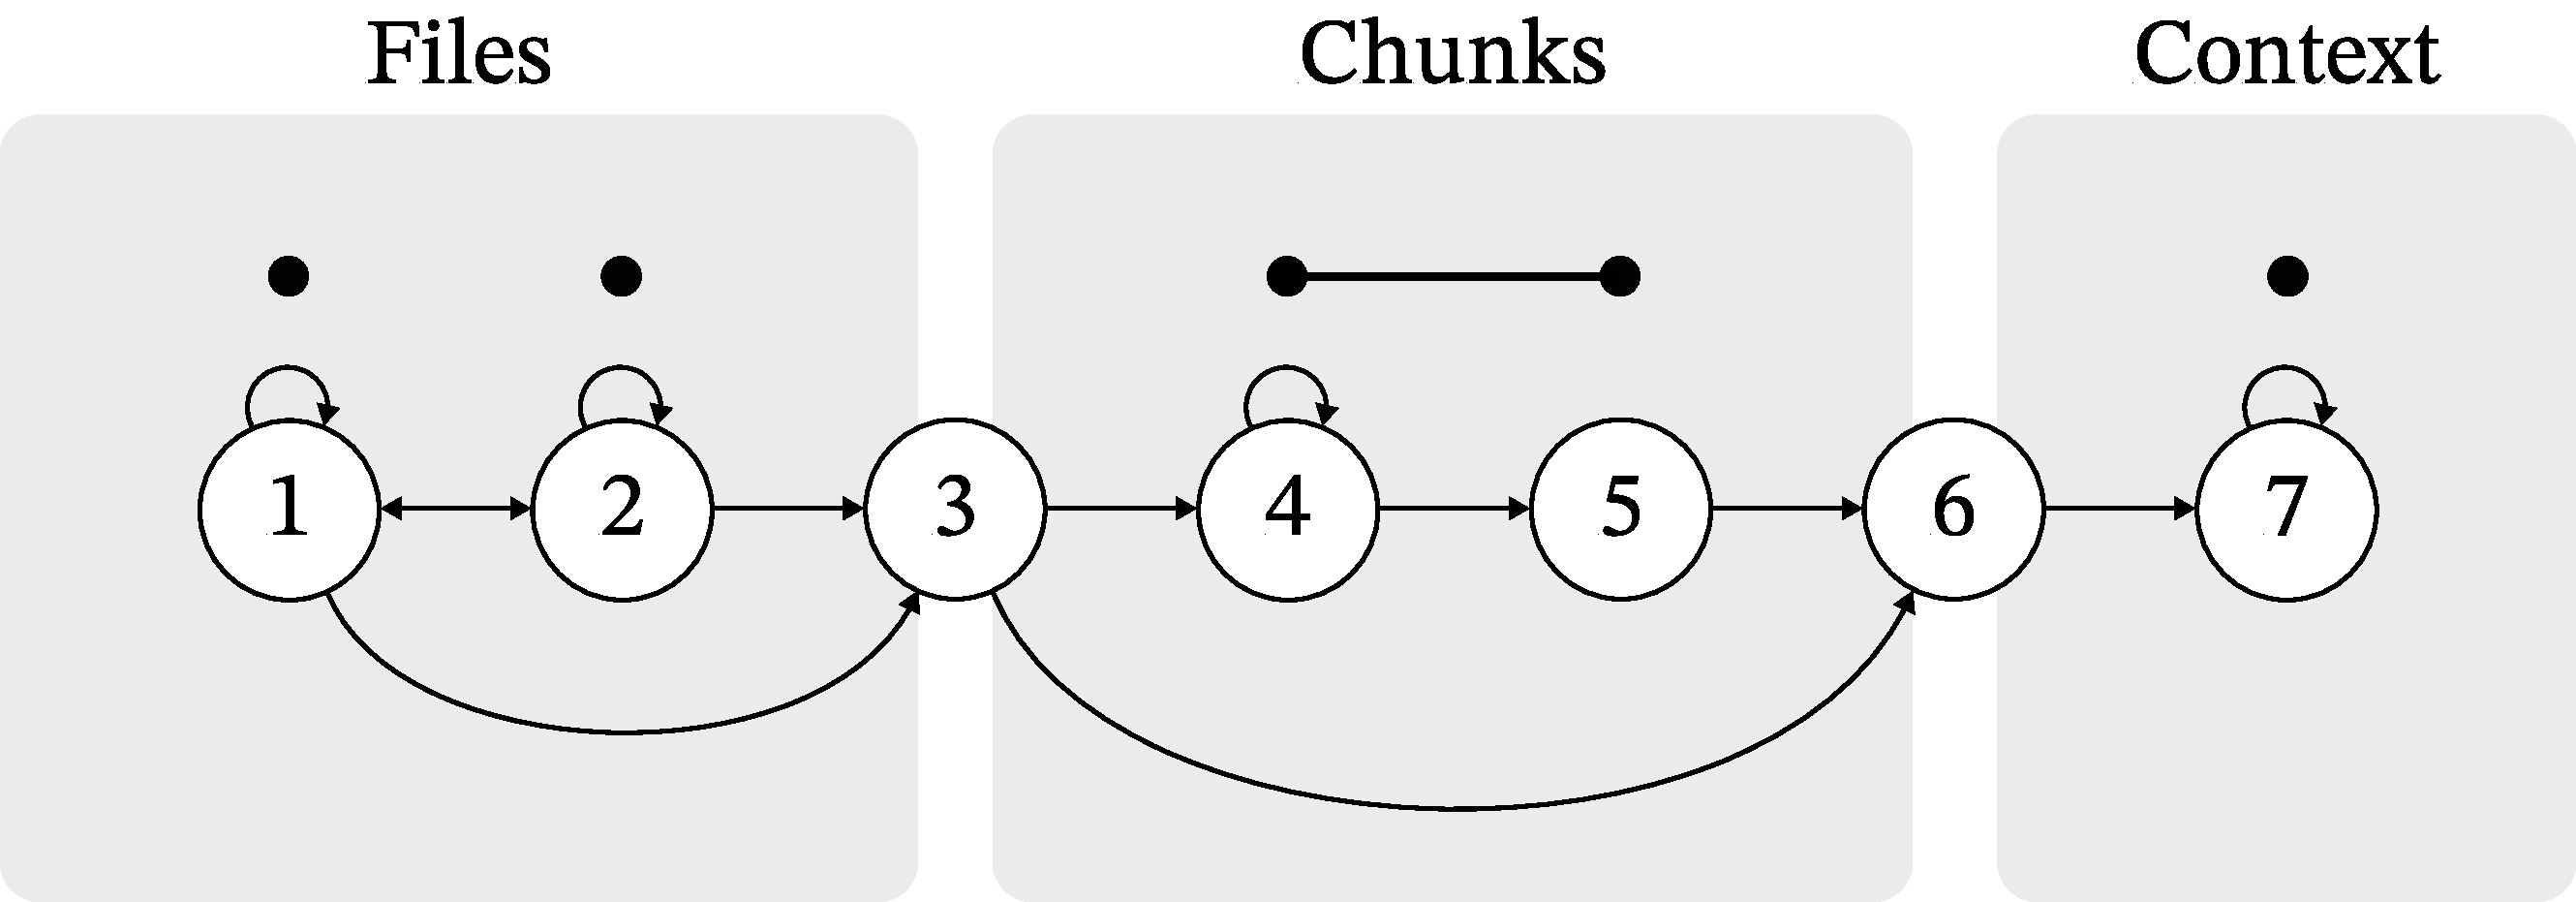
\includegraphics[width=\textwidth]{figures/composer-blocks.pdf}
    \shortcaption{Order of composer blocks}{Order of composer blocks. Nodes represent block types: \textcircled{\raisebox{-0.9pt}{1}} File Filtering, \textcircled{\raisebox{-0.9pt}{2}} File Preprocessing, \textcircled{\raisebox{-0.9pt}{3}} File Chunking, \textcircled{\raisebox{-0.9pt}{4}} Chunk Ranking, \textcircled{\raisebox{-0.9pt}{5}} Chunk Sorting, \textcircled{\raisebox{-0.9pt}{6}} Chunk Assembling, and \textcircled{\raisebox{-0.9pt}{7}} Context Postprocessing. Edges indicate the permissible sequence of block application. The data format is denoted by three frames: Files, Chunks, and Context. The bold subgraph highlights blocks that may be omitted.}\label{fig:composer-blocks}
\end{figure}

\subsection{List of Context Composers}\label{sec:context-composers-list}

\begin{sloppypar}
All context composers utilized in the \nameref{chap:research-investigation} chapter adhere to two standard preprocessing steps: the removal of empty files and the normalization of all line endings to the Line Feed character. These shared preprocessing steps ensure consistency across all experiments. We present the following list to provide a comprehensive overview of the context composers implemented and employed in this research, along with a justification of their design choices.
\end{sloppypar}

\begin{enumerate}
    \item \textbf{File-Level} produces an empty context. We use this composer as a baseline for comparison and to highlight the differences introduced by the repository context.
    \item \textbf{Path Distance} constructs the context using only files with the \texttt{.py} extension. The selected files are sorted in descending order according to their path distance from the completion file. For files with identical path distances, a secondary sorting criterion is applied using the Intersection over Union (IoU) metric, which equals to the number of lines shared with the completion file divided by the total number of unique lines in both files. The IoU calculation considers lines with leading and trailing whitespace removed and includes only those lines that are at least five characters in length after whitespace removal. We regard this composer as a representative of simple sparse RAG systems and designate it as a secondary baseline.
    \item \textbf{Lines IoU} is similar to the Path Distance method, but omits the initial sorting by path distance. Instead, files are ranked directly using the IoU metric. We add this composer to the framework as it expands upon the Path Distance and redefines its relevance function, thereby strengthening the grounding of the research conclusions.
    \item \textbf{Code Chunks} removes all docstrings, comments, and import statements from the context produced by Path Distance. We include this composer to assess the impact of non-functional code elements in context.
    \item \textbf{Half-Memory} begins with the context generated by Path Distance. Each line is independently removed with a dropout probability of \(0.5\), maintaining the overall saturation of the context window. By presenting this composer, we test the model's ability to extract useful information from dysfunctional code.
    \item \textbf{Declarations} extends Path Distance by filtering out all non-declarative elements, retaining only function and class declarations. We consider this composer to evaluate whether the declarations are sufficient to achieve a functional understanding of the code. It is important to note that this type of context includes a larger number of ICL demonstrations of inferior quality compared to Path Distance.
    \item \textbf{Text Chunks} uses Path Distance as the base composer, but removes all code from the context, leaving only docstrings and comments. We employ this composer to address the setting opposite to that of Code Chunks.
    \item \textbf{Text Files} constructs the context using files with the extensions \texttt{.json}, \texttt{.yaml}, \texttt{.yml}, \texttt{.sh}, \texttt{.md}, \texttt{.txt}, and \texttt{.rst}. The selected files are grouped in ascending order of relevance: [\texttt{.json}], [\texttt{.yaml}, \texttt{.yml}], [\texttt{.sh}], [\texttt{.md}, \texttt{.txt}, \texttt{.rst}]. Within each group, files are further sorted in descending order according to their path distance from the completion file. This composer enables us to assess the significance of the context based on standalone documentation and configuration files.
    \item \textbf{Random Files} constructs the context by randomly ordering all files from the repository snapshot. We introduce this composer to encompass the scenario of a non-empty repository context that is independent of the completion file.
    \item \textbf{Random \texttt{.py}} selects only files with the \texttt{.py} extension and arranges them in a random order. We design this composer to resemble Random Files, ensuring that it includes only inlier ICL demonstrations for the completion file.
    \item \textbf{Random Tokens} constructs the context by sampling a sequence of non-special tokens at random, with each token selected independently and with equal probability. We intend for this composer to test the model's robustness to such context and to represent the scenario of a full context window devoid of any (relevant) repository context.
    \item \textbf{Duplication} constructs the context by repeatedly concatenating the content of the completion file until the maximum context window size is reached. We utilize this composer as a sanity check for our experiments, to examine the effect of data leakage, and to evaluate the model's capability to copy ground-truth completions.
    \item \textbf{Leak} begins with the context produced by Path Distance. The completion file is randomly divided into five segments at newline characters, which then disjointedly replace context lines at random positions, approximately preserving the original token count. By including this composer, we inspect a more moderate data leakage scenario and evaluate the model's ability to extract ground-truth lines. \parencite{sapronov2025}
\end{enumerate}

\subsection{Order Modifications}

To increase the diversity of experiments conducted to address \hyperref[rq:rq-b1]{RQ.B1} and \hyperref[rq:rq-b2]{RQ.B2}, we consider two additional file ordering modifications alongside the \textit{original} mode, as illustrated in \figureref{fig:order-modes}:

\begin{itemize}
    \item \textit{reversed}: The retrieved files that fit within the model's context window are reordered in reverse. Consequently, the most relevant file appears at the beginning of the context window. We employ this mode to investigate the impact of demonstration permutations on ICL capabilities.
    \item \textit{irrelevant}: The order of retrieved files is reversed prior to the context length cut-off, resulting in a complete reversal of the context, with the most irrelevant files positioned at the end of the context string. It enables us to evaluate the significance of irrelevant repository context in light of our research questions.
\end{itemize}

\begin{figure}[ht]
    \centering
    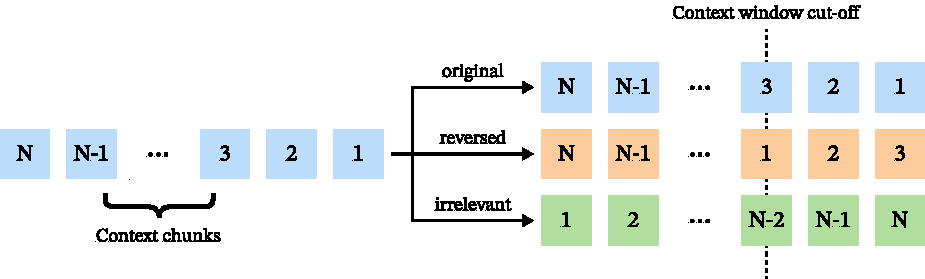
\includegraphics[width=\textwidth]{figures/order-modes.pdf}
    \shortcaption{Three modes of context ordering}{Three modes of context ordering. The numbers in boxes indicate the rank of the chunks, with smaller numbers denoting higher relevance.}\label{fig:order-modes}
\end{figure}

\subsection{Examples}

In addition to the blocks used to create composers employed in our experiments, we provide further exemplary implementations in the attached code, totaling 30 distinct blocks. The repository also includes a demonstrative Jupyter Notebook that describes these blocks and offers concrete usage examples of the package. We hope that this foundation advances further research in this area and enhances the clarity of our experiments.

\section{Training Data}

The dataset was provided by JetBrains Research, which initialized this project, and is based on the methodology outlined in \citet{bogomolov2024}. It was constructed by traversing the GitHub histories of Python repositories and applying permissive license filtering to sample completion files and their corresponding parent commits. Each data point consists of a pair: a list of Python completion files and a repository snapshot that captures the state of the repository at the time the completion files were added. The snapshot includes all text files except for the completion files themselves. To prevent contamination of the benchmark used in the evaluation, any repositories present in the benchmark were excluded from the training data.

To delineate the scope of this work, we ought to note that the corpus described thus far was entirely provided by JetBrains Research and was not generated by the author of this thesis. Conversely, the subsequent processing steps applied to this dataset represent the original contributions of the author.

We apply multiple filtering criteria to obtain the dataset with greater relevance and quality. First, all commits made prior to 2010 are excluded. Second, completion files with lengths outside the closed interval [800, 25000] characters are removed. Third, to eliminate redundancy, a simple deduplication strategy is employed on completion files based on the file name and the name of the repository to which they belong. Finally, up to 1000 of the most recently updated unique completion files are selected from each repository. The remaining repository snapshot is retained without additional processing. \parencite{sapronov2025}

The resulting corpus comprises 1,640 repositories, 160,801 commits, and 361,052 completion files. The completion files contain a total of 1.7 billion characters, while the repository snapshot files contain 4.8 trillion characters. To ensure the reproducibility of our research, we provide the identifiers for all data points within this corpus.

A subset of 2560 samples is randomly selected to form the validation set. During this process, we ensure that the repositories included in the training and validation sets do not overlap, and that no more than five different completion files are sourced from the same repository. After sampling for validation, the remaining data is sufficient to cover more than 250,000 unique completion files. We then apply the pre-composition procedure using the context composers listed in \sectionref{sec:context-composers-list}. This allows us to perform this operation only once and reuse the smaller produced datasets for several experiments. Moreover, instead of saving the entire context string, which can reach the length of the total number of characters used in the repository, we apply a 16K-token cut-off, ensuring that the resulting datasets range from 4 to 17 GB in Parquet format. A demonstration of the first five data points of each dataset is provided in the accompanying thesis repository.

It is important to note that the pre-composition of both the training and validation sets is based on the entire completion file. This approach is motivated by the inefficiency of selecting target lines to possess file prefixes during the training and validation processes. For better clarity, one can consider training on a single line from each completion file; this results in the degradation of the gradient approximation proportional to the number of completion lines, or an increase in the number of forward and backward passes to the same degree.

\section{Fine-Tuning Pipeline}

For the purposes of this research, we developed a fine-tuning pipeline aimed at adapting Code LLMs to the repository-level context.

From the data perspective, it supports the integration of pre-composed datasets obtained from the aforementioned context composition framework. We design the train-validation split to eliminate data leakage from samples gathered from the same repositories. By enabling configurable tokenization we ensure context window saturation and facilitate the application of gradient masking.

The pipeline integrates models from the Hugging Face Hub\footnote{\url{https://huggingface.co/}}. It supports adapters that can augment the model architecture, freeze a subset of parameters, or modify the optimizer initialization. Models are dynamically loaded onto a single device based on hardware availability. Efficient attention implementation and parameter data types are selected using the same principle.

We implement the training loop in pure PyTorch\footnote{\url{https://pytorch.org/}}, as it is a highly adaptable framework that provides a substantial level of flexibility and performance. The pipeline supports cosine learning rate scheduling with linear warmup, gradient scaling, clipping, and accumulation. The user can periodically invoke two validation loops: one on the original dataset split and another on an additional provided dataset. The latter allows metrics to be grounded on baseline composition strategy instead of solely monitoring the in-distribution capabilities of the model.

During the training process, the pipeline produces a set of configurable metrics and statistics for both the training and validation data. These include cross-entropy, Exact Match, Top-\(k\) Accuracy, learning rate tracking, epoch and token number counting. We log all these values to ensure adequate monitorability of the experiments. Furthermore, we decompose their values based on the types of tokens to which they are applied and denote these types as follows:
\begin{itemize}
    \item \textbf{Attached:} Tokens whose losses participate as leaf nodes in automatic differentiation for gradient computation.
    \item \textbf{Detached:} Tokens whose losses are zeroed out during gradient masking and serve as a complement to the attached tokens.
    \item \textbf{Completion:} Tokens of the completion file.
    \item \textbf{Context:} Tokens of the repository context.
    \item \textbf{Full:} All tokens.
\end{itemize}

In addition to statistics and metrics, the pipeline provides logging of the standard output and error streams. Checkpointing of the model and optimizer states is also supported.

The entire pipeline utilizes a modular structure, which enhances code maintainability and extendability. We design it in an end-to-end manner, requiring only a pre-composed dataset, a set of YAML configuration files, and a single command line from the user. We accompany all components that exhibit stochastic behavior with a seed parameter, ensuring the reproducibility of all experiments.

\section{Tools}

In the context composition framework, we integrate Hugging Face tokenizers from the Transformers\footnote{\url{https://github.com/huggingface/transformers}} library to compute token-related statistics, and Tree-sitter\footnote{\url{https://tree-sitter.github.io/tree-sitter/}} to decompose Python code into its parts. Both libraries are employed in the concrete implementations of the blocks, although their usage can be omitted without disrupting the main abstract framework. The OmegaConf\footnote{\url{https://github.com/omry/omegaconf}} configuration system is utilized to manage the initialization of the composers from YAML configuration files.

The pipeline inherits requirements from the context composition framework as it utilizes its functions. Additionally, we employ Datasets\footnote{\url{https://github.com/huggingface/datasets}} and Accelerate\footnote{\url{https://github.com/huggingface/accelerate}} from the Hugging Face ecosystem to provide peripheral support to the Transformers library. Pandas\footnote{\url{https://github.com/pandas-dev/pandas}} is used to load pre-composed datasets from the Parquet format. We extend the configurative capabilities of OmegaConf and enhance the pipeline's usability by using the Hydra\footnote{\url{https://github.com/facebookresearch/hydra}} package. PyTorch, as mentioned in the previous section, is utilized to implement the training loop. The tqdm\footnote{\url{https://github.com/tqdm/tqdm}} library is employed to display progress bars for all prolonged processes. Weights~\&~Biases\footnote{\url{https://github.com/wandb/wandb}} is used to track metrics and statistics in real-time.

We use a single 8\(\times\)H200 node, with each GPU possessing 141 GB of VRAM, to conduct all experiments and execute evaluation script.
